\subsection{Tích hợp và Ứng dụng}
\label{subsec:integration}
\textcolor{orange}{Quang Minh, Chí Nguyên}

Subsection này đóng vai trò tổng hợp, nơi các thành phần của QNN được kết nối để tạo thành một mô hình hoàn chỉnh. Chúng tôi áp dụng QNN cho bài toán phân loại nhị phân Two-Moon nhằm minh họa toàn bộ quy trình từ mã hóa dữ liệu đến huấn luyện và đánh giá mô hình.

%=============================================================================
\subsubsection{Bài toán Two-Moon Classification}
%=============================================================================

Bài toán Two-Moon là một bài toán phân loại nhị phân kinh điển, trong đó dữ liệu được phân bố theo hai hình bán nguyệt lồng vào nhau. Đây là bài toán phi tuyến tính, đòi hỏi mô hình phải học được ranh giới quyết định phức tạp.

Dữ liệu được sinh ra bằng hàm \texttt{make\_moons} từ thư viện scikit-learn với các cấu hình sau:

\begin{table}[H]
\centering
\caption{Cấu hình thí nghiệm cho bộ dữ liệu Two-Moon}
\label{tab:dataset_config}
\begin{tabular}{|l|l|}
\hline
\textbf{Tham số} & \textbf{Giá trị} \\
\hline
Kích thước mẫu (Sample sizes) & 1,000 và 10,000 \\
\hline
Mức nhiễu (Noise levels) & 0.1, 0.5, 0.9 \\
\hline
Tỷ lệ Train/Validation & 75\% / 25\% \\
\hline
Random seed & 42 \\
\hline
\end{tabular}
\end{table}

Mỗi lớp (Class 0 và Class 1) có số lượng mẫu cân bằng (50\% mỗi lớp). Hình \ref{fig:dataset_distribution} minh họa phân bố dữ liệu với các mức nhiễu khác nhau.

\begin{figure}[H]
\centering
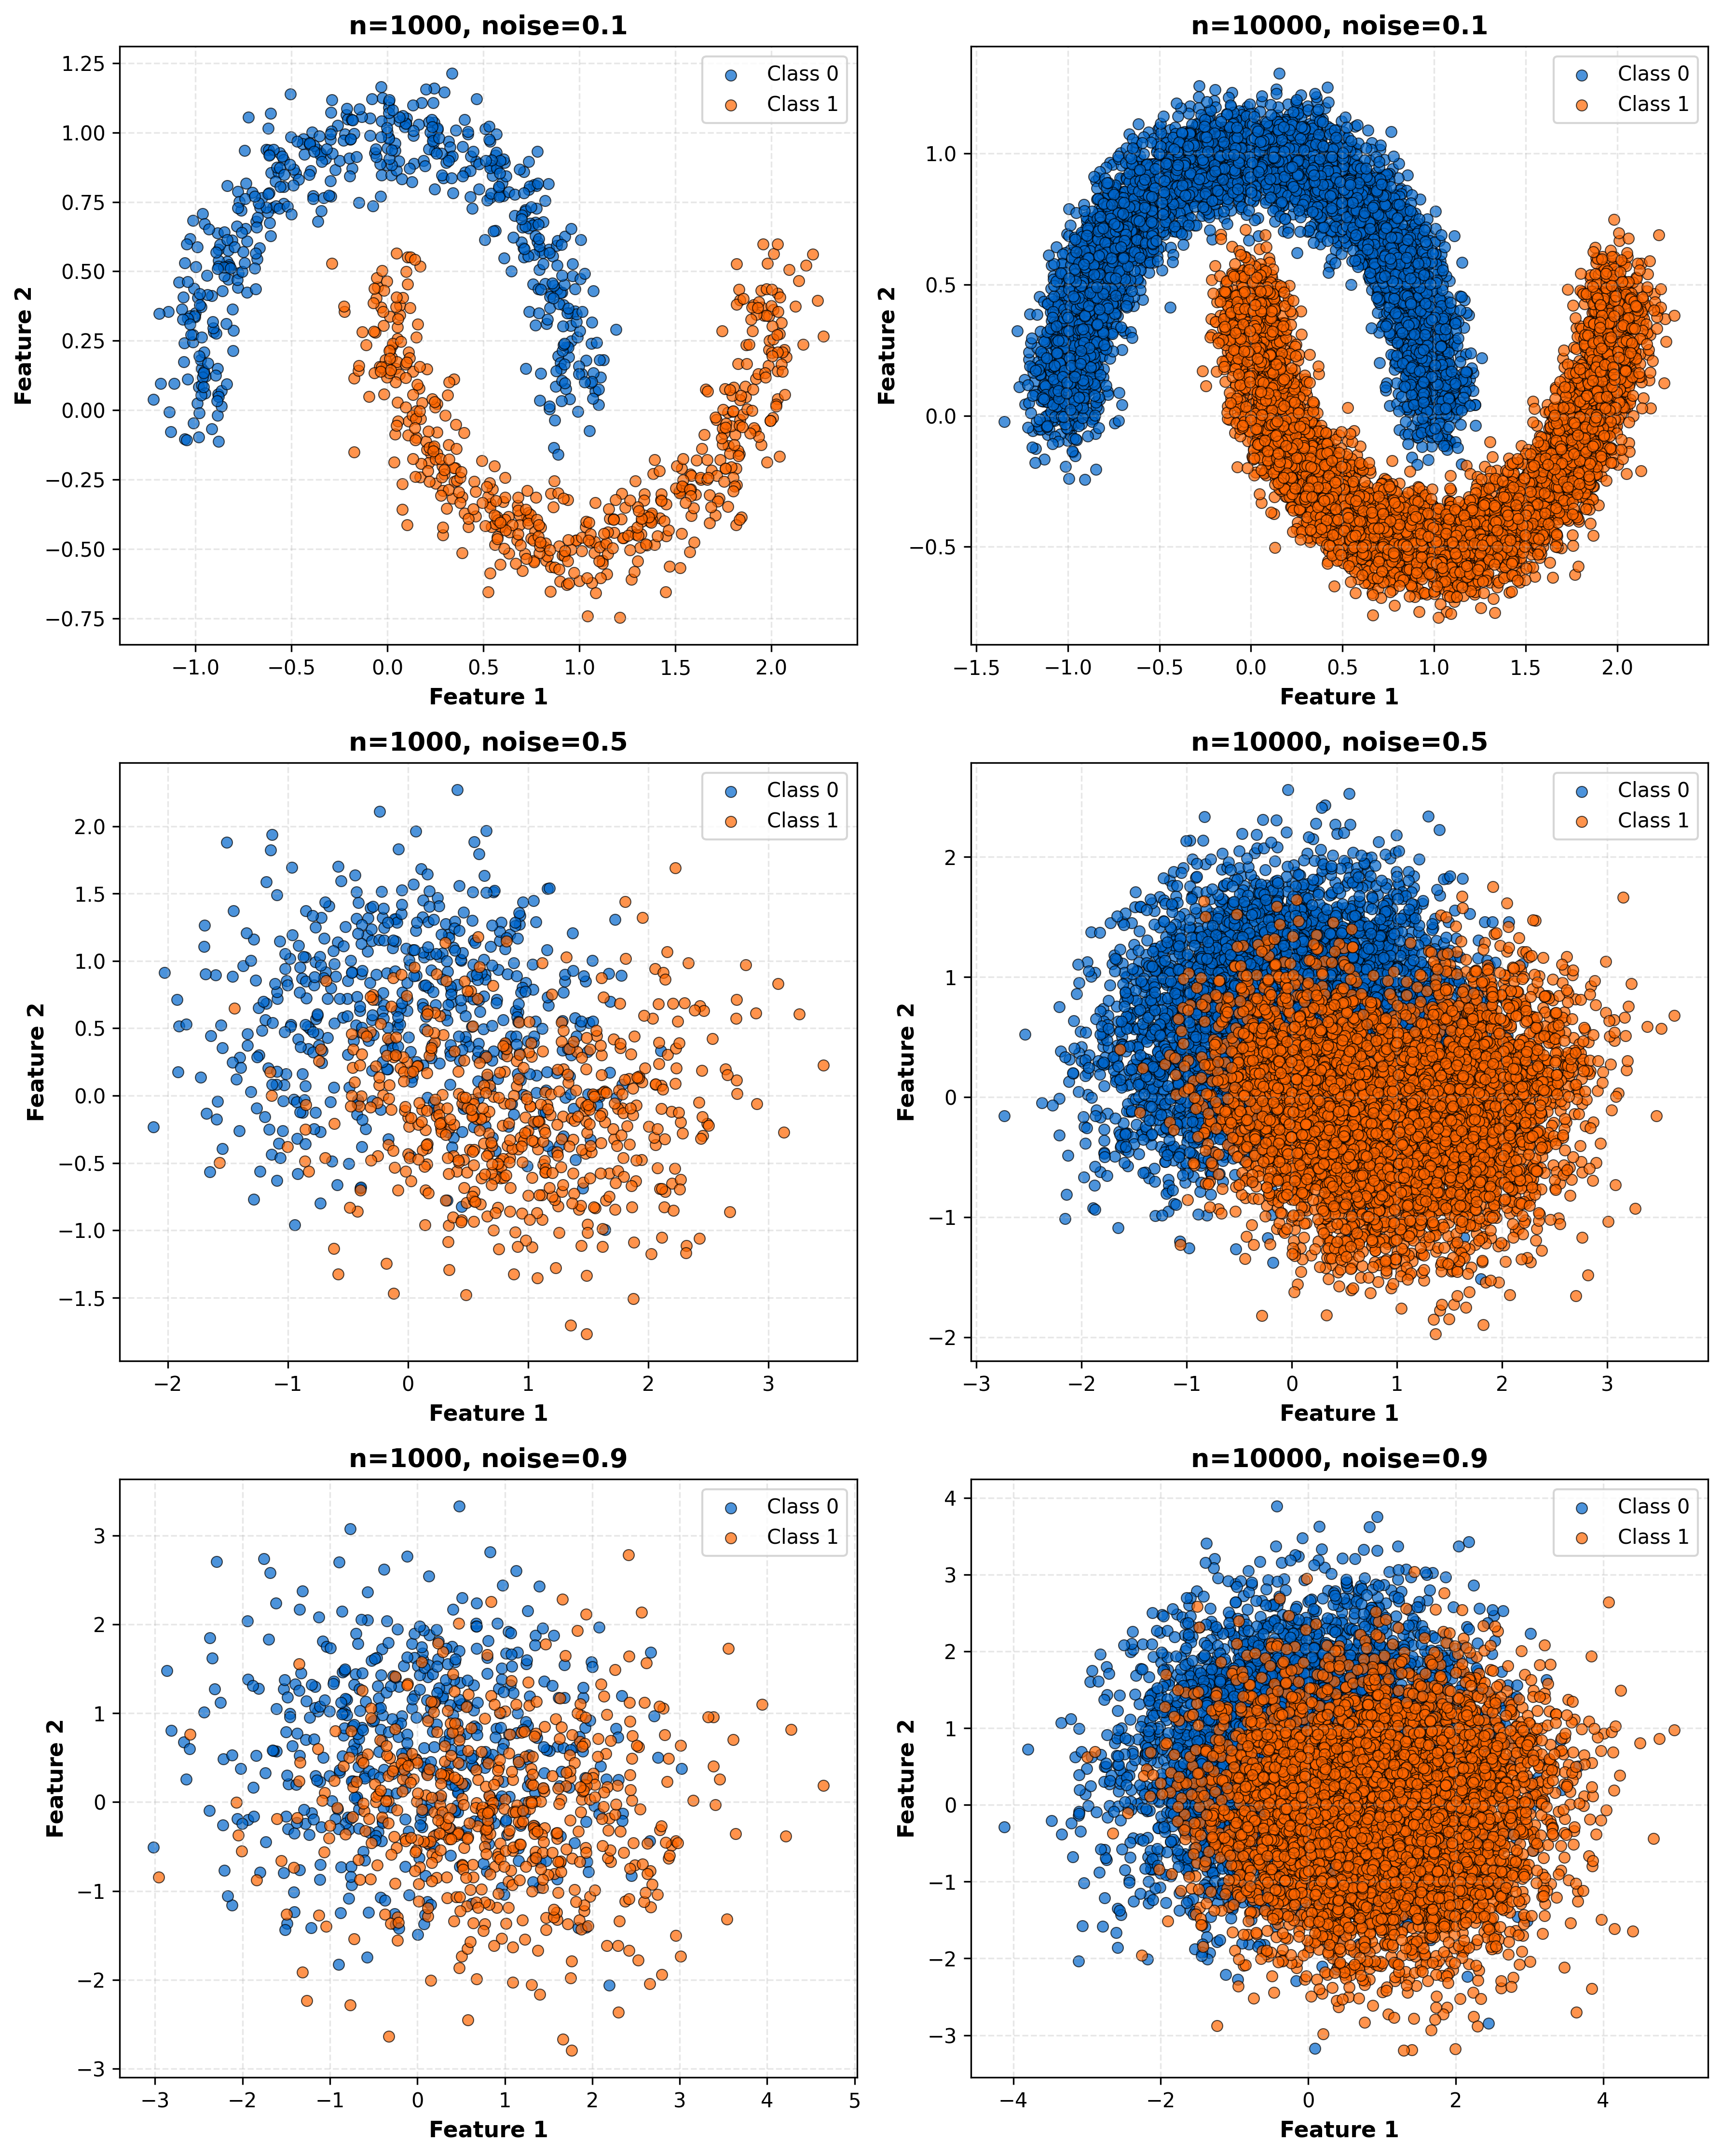
\includegraphics[width=\textwidth]{figures/dataset_distribution.png}
\caption{Phân bố dữ liệu Two-Moon với các kích thước mẫu (n=1000, n=10000) và mức nhiễu khác nhau (noise=0.1, 0.5, 0.9). Khi mức nhiễu tăng, ranh giới giữa hai lớp trở nên mờ hơn, làm tăng độ khó của bài toán phân loại.}
\label{fig:dataset_distribution}
\end{figure}

\begin{figure}[H]
\centering
\includegraphics[width=\textwidth]{figures/gaussian_analysis.png}
\caption{Phân tích phân phối Gaussian của các đặc trưng. Histogram cho thấy phân phối của Feature 1 và Feature 2 với đường cong Gaussian fit, thể hiện các tham số $\mu$ (mean) và $\sigma$ (standard deviation).}
\label{fig:gaussian_analysis}
\end{figure}

%=============================================================================
\subsubsection{Pipeline hoàn chỉnh của QNN}
%=============================================================================

Mô hình Quantum Neural Network (QNN) được xây dựng theo kiến trúc hybrid quantum-classical với pipeline như sau:

\begin{enumerate}
    \item \textbf{Lớp đầu vào cổ điển (Input Layer):} Biến đổi dữ liệu từ không gian 2 chiều sang không gian $n$-qubit
    \begin{equation}
        \mathbf{x}' = W_{in} \cdot \mathbf{x} + \mathbf{b}_{in}
    \end{equation}
    trong đó $W_{in} \in \mathbb{R}^{n_{qubits} \times 2}$ và $\mathbf{b}_{in} \in \mathbb{R}^{n_{qubits}}$.
    
    \item \textbf{Mã hóa lượng tử (Angle Embedding):} Mã hóa dữ liệu cổ điển vào trạng thái lượng tử
    \begin{equation}
        |\psi(\mathbf{x}')\rangle = \bigotimes_{i=0}^{n-1} R_Y(x'_i)|0\rangle
    \end{equation}
    
    \item \textbf{Mạch lượng tử tham số (Variational Circuit):} Sử dụng BasicEntanglerLayers với cổng CNOT để tạo entanglement
    \begin{equation}
        U(\boldsymbol{\theta}) = \prod_{l=1}^{L} \left[ \prod_{i=0}^{n-1} R_Y(\theta_{l,i}) \cdot \text{CNOT}_{ring} \right]
    \end{equation}
    trong đó $L$ là số layers và $\text{CNOT}_{ring}$ kết nối các qubit theo cấu trúc vòng.
    
    \item \textbf{Đo lường (Measurement):} Đo giá trị kỳ vọng của Pauli-Z trên mỗi qubit
    \begin{equation}
        z_i = \langle \psi | Z_i | \psi \rangle, \quad i = 0, 1, ..., n-1
    \end{equation}
    
    \item \textbf{Lớp đầu ra cổ điển (Output Layer):} Biến đổi kết quả đo thành logits cho 2 lớp
    \begin{equation}
        \mathbf{y} = W_{out} \cdot \mathbf{z} + \mathbf{b}_{out}
    \end{equation}
\end{enumerate}

\begin{figure}[H]
\centering
\begin{tikzpicture}[node distance=2cm, auto]
    % Nodes
    \node[draw, rectangle, minimum width=2.5cm, minimum height=1cm] (input) {Input Layer\\$\mathbb{R}^2 \to \mathbb{R}^n$};
    \node[draw, rectangle, minimum width=2.5cm, minimum height=1cm, right=of input] (encoding) {Angle\\Embedding};
    \node[draw, rectangle, minimum width=2.5cm, minimum height=1cm, right=of encoding] (var) {Variational\\Circuit};
    \node[draw, rectangle, minimum width=2.5cm, minimum height=1cm, right=of var] (measure) {Measurement\\$\langle Z \rangle$};
    \node[draw, rectangle, minimum width=2.5cm, minimum height=1cm, right=of measure] (output) {Output Layer\\$\mathbb{R}^n \to \mathbb{R}^2$};
    
    % Arrows
    \draw[->] (input) -- (encoding);
    \draw[->] (encoding) -- (var);
    \draw[->] (var) -- (measure);
    \draw[->] (measure) -- (output);
    
    % Labels
    \node[above=0.3cm of input] {\small Classical};
    \node[above=0.3cm of encoding] {\small Quantum};
    \node[above=0.3cm of var] {\small Quantum};
    \node[above=0.3cm of measure] {\small Quantum};
    \node[above=0.3cm of output] {\small Classical};
\end{tikzpicture}
\caption{Pipeline của mô hình Hybrid Quantum Neural Network}
\label{fig:qnn_pipeline}
\end{figure}

%=============================================================================
\subsubsection{Triển khai mô hình bằng PennyLane}
%=============================================================================

Mô hình được triển khai sử dụng framework PennyLane kết hợp với PyTorch. Dưới đây là code triển khai mạch lượng tử:

\begin{lstlisting}[language=Python, caption={Định nghĩa mạch lượng tử và mô hình hybrid}, label={lst:quantum_model}]
import pennylane as qml
import torch.nn as nn

def create_quantum_model(n_qubits=2, n_layers=6):
    # Create quantum device (simulator)
    backend = qml.device("default.qubit", wires=n_qubits)
    
    # Define quantum circuit
    @qml.qnode(backend)
    def qnode(inputs, weights):
        # Angle Embedding: encode classical data
        qml.templates.AngleEmbedding(inputs, wires=range(n_qubits))
        # Variational layers with entanglement
        qml.templates.BasicEntanglerLayers(weights, wires=range(n_qubits))
        # Measure expectation values
        return [qml.expval(qml.PauliZ(wires=i)) for i in range(n_qubits)]
    
    # Create quantum layer for PyTorch
    weight_shapes = {"weights": (n_layers, n_qubits)}
    qlayer = qml.qnn.TorchLayer(qnode, weight_shapes)
    
    # Define hybrid model
    class HybridModel(nn.Module):
        def __init__(self):
            super().__init__()
            self.input_layer = nn.Linear(2, n_qubits)
            self.qlayer = qlayer
            self.output_layer = nn.Linear(n_qubits, 2)
            
        def forward(self, x):
            x = self.input_layer(x)
            x = self.qlayer(x)
            x = self.output_layer(x)
            return x
    
    return HybridModel()
\end{lstlisting}

\paragraph{Khám phá kiến trúc lượng tử tối ưu}

Trước khi so sánh với các mô hình cổ điển, chúng tôi tiến hành khám phá các cấu hình kiến trúc lượng tử khác nhau để tìm ra cấu hình tối ưu:

\begin{table}[H]
\centering
\caption{Kết quả khám phá kiến trúc Quantum với 1000 mẫu, noise=0.1}
\label{tab:quantum_arch}
\begin{tabular}{|c|c|c|c|c|}
\hline
\textbf{Cấu hình} & \textbf{Số Qubits} & \textbf{Số Layers} & \textbf{Accuracy} & \textbf{Training Time} \\
\hline
Q2L2 & 2 & 2 & 0.8830 & 9.02s \\
Q2L4 & 2 & 4 & 0.8830 & 13.64s \\
Q2L6 & 2 & 6 & 0.9930 & 18.62s \\
Q3L2 & 3 & 2 & \textbf{0.9940} & 14.70s \\
Q3L4 & 3 & 4 & 0.9890 & 19.64s \\
Q3L6 & 3 & 6 & 0.8790 & 26.41s \\
\hline
\end{tabular}
\end{table}

\textbf{Kết quả:} Cấu hình tối ưu là \textbf{Q3L2} (3 qubits, 2 layers) với accuracy 99.40\%. Đáng chú ý, việc tăng số layers không luôn cải thiện kết quả - Q3L6 thực sự cho kết quả kém hơn Q3L2, có thể do overfitting hoặc barren plateau.

%=============================================================================
\subsubsection{Cấu hình huấn luyện}
%=============================================================================

\begin{table}[H]
\centering
\caption{Các hyperparameter cho quá trình huấn luyện}
\label{tab:training_config}
\begin{tabular}{|l|c|}
\hline
\textbf{Hyperparameter} & \textbf{Giá trị} \\
\hline
Số epochs & 10 \\
Batch size & 5 \\
Learning rate & 0.05 \\
Optimizer & Adam \\
Loss function & Cross-Entropy \\
Train/Val split & 75\%/25\% \\
\hline
\end{tabular}
\end{table}

%=============================================================================
\subsubsection{Các mô hình học máy cổ điển để so sánh}
%=============================================================================

Để đánh giá công bằng, tất cả các mô hình cổ điển đều được triển khai dưới dạng neural networks sử dụng PyTorch:

\begin{table}[H]
\centering
\caption{Kiến trúc các mô hình cổ điển}
\label{tab:classical_models}
\begin{tabular}{|l|l|l|}
\hline
\textbf{Mô hình} & \textbf{Kiến trúc} & \textbf{Số tham số (approx)} \\
\hline
Classical NN & Linear(2→8→4→2) + ReLU & 58 \\
Logistic Regression & Linear(2→2) & 6 \\
SVM (RBF approx) & Linear(2→20→2) + ReLU & 82 \\
Decision Tree & Linear(2→16→8→2) + ReLU & 186 \\
Random Forest & Ensemble of 10 trees (2→8→2) & 340 \\
Naive Bayes & Linear(2→4→2) + ReLU & 22 \\
AdaBoost & Ensemble of 10 estimators (2→4→2) & 220 \\
\hline
Quantum NN (Q3L2) & Input(2→3) + QCircuit(3×2) + Output(3→2) & 17 \\
\hline
\end{tabular}
\end{table}

%=============================================================================
\subsubsection{So sánh kết quả thực nghiệm}
%=============================================================================

\paragraph{Kết quả với 1,000 mẫu}

\begin{table}[H]
\centering
\caption{So sánh accuracy các mô hình với n=1,000 samples}
\label{tab:results_1000}
\begin{tabular}{|l|c|c|c|c|c|c|}
\hline
\textbf{Model} & \multicolumn{2}{c|}{\textbf{noise=0.1}} & \multicolumn{2}{c|}{\textbf{noise=0.5}} & \multicolumn{2}{c|}{\textbf{noise=0.9}} \\
\cline{2-7}
 & Acc & Time(s) & Acc & Time(s) & Acc & Time(s) \\
\hline
Random Forest & \textbf{1.0000} & 3.94 & \textbf{0.8080} & 7.46 & 0.7120 & 7.01 \\
Classical NN & 0.9990 & 1.04 & 0.8030 & 1.59 & 0.5000 & 1.58 \\
Decision Tree & 0.9990 & 0.94 & 0.7940 & 1.93 & 0.6850 & 1.53 \\
AdaBoost & 0.9990 & 4.03 & 0.8050 & 6.44 & 0.7030 & 7.31 \\
SVM & 0.9980 & 0.78 & 0.7930 & 1.34 & 0.6750 & 1.24 \\
Naive Bayes & 0.9920 & 0.97 & 0.7990 & 1.24 & 0.6780 & 1.38 \\
Logistic Reg. & 0.8770 & 0.59 & 0.7780 & 0.93 & \textbf{0.7140} & 0.86 \\
\rowcolor{green!20}
Quantum NN & 0.8760 & 13.13 & 0.7810 & 21.25 & 0.6630 & 21.41 \\
\hline
\end{tabular}
\end{table}

\paragraph{Kết quả với 10,000 mẫu}

\begin{table}[H]
\centering
\caption{So sánh accuracy các mô hình với n=10,000 samples}
\label{tab:results_10000}
\begin{tabular}{|l|c|c|c|c|c|c|}
\hline
\textbf{Model} & \multicolumn{2}{c|}{\textbf{noise=0.1}} & \multicolumn{2}{c|}{\textbf{noise=0.5}} & \multicolumn{2}{c|}{\textbf{noise=0.9}} \\
\cline{2-7}
 & Acc & Time(s) & Acc & Time(s) & Acc & Time(s) \\
\hline
\rowcolor{green!20}
Quantum NN & \textbf{0.9992} & 222.07 & 0.8195 & 216.11 & 0.7263 & 223.40 \\
Decision Tree & 0.9985 & 16.37 & 0.8132 & 16.41 & 0.6966 & 16.42 \\
Random Forest & 0.9979 & 65.59 & \textbf{0.8221} & 68.93 & 0.7258 & 68.96 \\
Classical NN & 0.9950 & 16.54 & 0.8171 & 16.30 & 0.5000 & 16.35 \\
SVM & 0.9950 & 12.88 & 0.8193 & 12.99 & 0.7211 & 13.00 \\
AdaBoost & 0.9901 & 64.90 & 0.8218 & 101.08 & \textbf{0.7263} & 101.30 \\
Naive Bayes & 0.9631 & 12.16 & 0.8043 & 12.14 & 0.7000 & 12.09 \\
Logistic Reg. & 0.8850 & 8.53 & 0.7879 & 8.56 & 0.7186 & 8.53 \\
\hline
\end{tabular}
\end{table}

\begin{figure}[H]
\centering
\includegraphics[width=\textwidth]{figures/accuracy_comparison.png}
\caption{So sánh accuracy giữa các mô hình trên các cấu hình khác nhau. Quantum NN (màu xanh lá) cho thấy hiệu suất vượt trội với dữ liệu lớn (n=10,000) và nhiễu thấp (noise=0.1), đạt accuracy cao nhất 99.92\%.}
\label{fig:accuracy_comparison}
\end{figure}

%=============================================================================
\subsubsection{Phân tích thời gian huấn luyện Quantum NN}
%=============================================================================

\begin{table}[H]
\centering
\caption{Chi tiết thời gian huấn luyện Quantum NN}
\label{tab:qnn_time}
\begin{tabular}{|c|c|c|c|c|c|}
\hline
\textbf{n\_samples} & \textbf{noise} & \textbf{Encoding} & \textbf{Pure Training} & \textbf{Inference} & \textbf{Total} \\
\hline
1,000 & 0.1 & 0.095s (0.7\%) & 13.04s (99.3\%) & 0.006s & 13.14s \\
1,000 & 0.5 & 0.085s (0.4\%) & 21.16s (99.6\%) & 0.007s & 21.26s \\
1,000 & 0.9 & 0.090s (0.4\%) & 21.32s (99.6\%) & 0.008s & 21.41s \\
10,000 & 0.1 & 0.214s (0.1\%) & 221.85s (99.9\%) & 0.020s & 222.09s \\
10,000 & 0.5 & 0.174s (0.1\%) & 215.93s (99.9\%) & 0.018s & 216.13s \\
10,000 & 0.9 & 0.173s (0.1\%) & 223.23s (99.9\%) & 0.019s & 223.42s \\
\hline
\end{tabular}
\end{table}

\textbf{Nhận xét:} Phần lớn thời gian huấn luyện (>99\%) là do quá trình tính gradient và cập nhật tham số (Pure Training), trong khi thời gian mã hóa dữ liệu (Encoding) chiếm tỷ lệ rất nhỏ (<1\%).

\begin{figure}[H]
\centering
\includegraphics[width=\textwidth]{figures/training_time_comparison.png}
\caption{So sánh thời gian huấn luyện giữa các mô hình. Quantum NN yêu cầu thời gian huấn luyện lớn hơn đáng kể so với các mô hình cổ điển do chi phí tính toán của mạch lượng tử.}
\label{fig:training_time}
\end{figure}

%=============================================================================
\subsubsection{Đường cong học tập (Learning Curves)}
%=============================================================================

\begin{figure}[H]
\centering
\includegraphics[width=\textwidth]{figures/learning_curves.png}
\caption{Đường cong học tập của các mô hình với n=1000, noise=0.1. Mỗi hàng hiển thị một mô hình với Loss và Accuracy cho cả Training (trái) và Validation (phải).}
\label{fig:learning_curves}
\end{figure}

%=============================================================================
\subsubsection{Ranh giới quyết định (Decision Boundaries)}
%=============================================================================

\begin{figure}[H]
\centering
\includegraphics[width=\textwidth]{figures/decision_boundaries.png}
\caption{Ranh giới quyết định của các mô hình trên tất cả các cấu hình. Quantum NN tạo ra ranh giới quyết định mượt mà và có khả năng khái quát hóa tốt, đặc biệt với dữ liệu nhiễu thấp.}
\label{fig:decision_boundaries}
\end{figure}

%=============================================================================
\subsubsection{Thảo luận và Kết luận}
%=============================================================================

\paragraph{Ưu điểm của Quantum Neural Network:}
\begin{itemize}
    \item \textbf{Hiệu suất cao với dữ liệu lớn:} Với n=10,000 và noise=0.1, QNN đạt accuracy cao nhất (99.92\%), vượt trội so với tất cả các mô hình cổ điển.
    \item \textbf{Số tham số ít:} QNN chỉ cần 17 tham số so với hàng trăm tham số của các mô hình ensemble như Random Forest.
    \item \textbf{Ranh giới quyết định mượt:} QNN tạo ra decision boundary mượt mà, tránh overfitting.
\end{itemize}

\paragraph{Hạn chế:}
\begin{itemize}
    \item \textbf{Thời gian huấn luyện dài:} QNN yêu cầu thời gian huấn luyện lớn hơn 10-20 lần so với các mô hình cổ điển.
    \item \textbf{Hiệu suất kém với nhiễu cao:} Với noise=0.9, QNN không phải là lựa chọn tốt nhất.
    \item \textbf{Hiệu suất kém với dữ liệu nhỏ:} Với n=1,000, các mô hình cổ điển như Random Forest thường cho kết quả tốt hơn.
\end{itemize}

\paragraph{Kết luận:}
Quantum Neural Network thể hiện tiềm năng vượt trội trong các bài toán với:
\begin{enumerate}
    \item Dữ liệu có kích thước lớn (n ≥ 10,000)
    \item Mức nhiễu thấp đến trung bình (noise ≤ 0.5)
    \item Yêu cầu mô hình compact với ít tham số
\end{enumerate}

Tuy nhiên, chi phí tính toán cao vẫn là rào cản chính cho việc ứng dụng QNN trong thực tế. Với sự phát triển của phần cứng lượng tử, những hạn chế này được kỳ vọng sẽ được giải quyết trong tương lai.

\begin{table}[H]
\centering
\caption{Tóm tắt: Mô hình tốt nhất cho từng cấu hình}
\label{tab:best_models_summary}
\begin{tabular}{|c|c|l|c|}
\hline
\textbf{n\_samples} & \textbf{noise} & \textbf{Best Model} & \textbf{Accuracy} \\
\hline
1,000 & 0.1 & Random Forest & 1.0000 \\
1,000 & 0.5 & Random Forest & 0.8080 \\
1,000 & 0.9 & Logistic Regression & 0.7140 \\
\rowcolor{green!20}
10,000 & 0.1 & \textbf{Quantum NN} & \textbf{0.9992} \\
10,000 & 0.5 & Random Forest & 0.8221 \\
10,000 & 0.9 & AdaBoost / Quantum NN & 0.7263 \\
\hline
\end{tabular}
\end{table}
